





%iso morphic src jos ei käy niin käytä tätä
%https://web.archive.org/web/20221206181248/https://old.gigaom.com/2014/12/27/meteor-wants-to-be-the-warp-drive-for-building-real-time-apps/
% Jonathan Vanian




MeteorJS on avoimeen lähdekoodiin perustuva full-stack JavaScript web-kehys, joka on 
suunniteltu nopeaan käyttöönottoon ja kehittämiseen eri laitteille\labciteend{meteor24b}
Meteor mahdollistaa isomorphisen koodin kirjoittamisen, eli koodiin, joka on samanlaista palvelimella sekä selaimella\labciteend{Kuster23} % en tiedä onko hyvä src mutta on totta joten pitäis löytää jokue
Meteor ei määritä käytettyä front-end teknologiaa vaan sillä on integraatio moneen yleiseen front-end framework:kiin, kuten Vue, React, Svelte tai Angular\labciteend{meteor24a}{}
%Tämä antaa lisäjoustoa Meteorille, sillä se antaa mahdollisuuden monelle sovelluskehittäjälle, joilla ei ole kokemusta tietystä front-end teknologiasta.\\
\medskip



    

Lisäksi Meteor \labcite{meteor24a}:
\begin{itemize}
    \item Tukee montaa Front-end kirjastoa ja frameworkkia.
    \item Tukee Typescriptiä.
    \item Rakentaa sisään käyttäjäpaketin.
    \item Toimii monella laitteella.
\end{itemize}
\medskip


Meteorin nopea käyttöönotto johtuu sen pakettijärjestelmästä ja valmiiksi asennetuista paketeista, kuten Meteorin käyttäjät-paketti. 
%Meteorin nopea käyttöönotto on osa johtuen sen paketti järjestelmästä ja valmiiksi paketoiduista paketeista, kuten Meteorin käyttäjät paketti. 
Käyttäjät-paketin avulla kehittäjä voi nopeasti luoda todennusjärjestelmän (eng authentication system),
joka antaa helpon integraation muiden palveluntarjoajien todennuspalvelujen kanssa kuten Facebook, GitHub, Google ym.
Käyttäjät-paketti on myös integroitu muihin Meteorin ominaisuuksiin kuten metodeihin.\labcite{meteor24c}



\subsubsection{Meteor-metodit}

% toinen kappale
% metodi tekee koodista yksinkertaisemman. metodi tekee rajapinnasta helpomman lukea sillä

% mahdollinen kappale rike kolmannessa kappaleessa


Meteor käyttää etäkäsittelykutsu-rajapintaa (eng Remote procedure call) perinteisen RESTful rajapinnan sijasta\labciteend{meteor24a}
Etäkäsittelykutsumallissa asiakasohjelma lähettää palvelinohjelmalle kutsuviestin.
Palvelinohjelma käsittelee kutsuviestin ja suorittaa halutun toiminnon ja palauttaa vastausviestin asiakasohjelmalle.\labcite{ibm23}
Meteorin metodit kokonaisuus toimii etäkäsittelykutsu-rajapintana selaimen ja palvelimen välillä. 
\medskip



Meteorin etäkäsittelykutsu metodit ovat palvelimella määriteltyjä funktioita, joita pystytään kutsumaan Meteorin kautta selaimelta tai palvelimelta. 
Kuvassa \nextImageCount{} on esimerkki Meteor metodin määritelmästä.
Metodit tekevät myös käyttöliittymäkoodista yksinkertaisemman, 
sillä metodien etäkäsittelukutsumalli poistaa käyttöliittymä koodista tarpeen tehdä GET tai POST pyyntöjä palvelimelle.
Metodi funktio käyttää JavaScriptin "this"{} ominaisuutta, jonka
avulla metodiin voidaan antaa kontekstia kutsujasta.
Tässä kontekstissa voi selvittää esimerkiksi onko kutsuja kirjautunut sisään, tai onko kutsujalla oikeat oikeudet kutsua metodia helpottaen turvallisuuden lisäämistä rajapintaan.
\bigskip

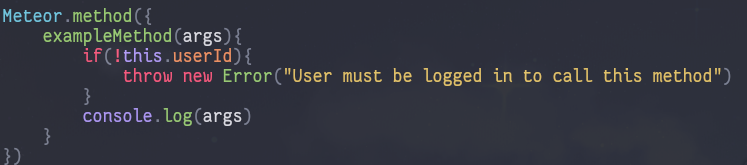
\includegraphics[width=15cm]{src/public/methodexample.png}\\
Kuva \getImgCount {}. Meteor-metodin määritelmä
\medskip

Kuvassa on Meteor metodin määritelmä "exampleMethod"{}, joka selvittää, onko "this"{} objektissa käyttäjätunnus ominaisuutta, 
näin metodi voi tietää onko kutsuja kirjautunut sisään,
jos käyttäjä ei ole kirjautunut sisään funktio aiheuttaa poikkeuksen, joka välitetään kutsujalle.
Jos käyttäjä on kirjautunut sisään, metodi tulostaa argumentit objektin. 
\medskip


%voidaan myös laittaa kuva metodi kutsusta jos halutaan


\subsubsection{Meteor-ecosysteemi}

%build system pitää vissii vähä paremmin selittää...
% sdelitetäänkö build system vai.... vaihdetaanko sana johonkin toiseen vaa


Meteor ylläpitää omaa paketointi ekosysteemiään. 
%nämä paketit ovat isomorphisia, eli ne toimivat palvelimella ja selaimella\labciteend{pranav17}{}
Meteorilla on itse Meteor tiimin ylläpitämiä paketteja ja kolmannen osapuolen paketteja,
joita yhteisö ylläpitää. Nämä kolmannen osapuolen paketit voi ladata Meteorin pakettipalvelimelle Athmosphere:lle.\labcite{sanders15}\\
\medskip


Athmosphere on Meteorin ylläpitämä pakettipalvelin, johon käyttäjät voivat ladata paketteja tai kirjastoja,
jotka ovat suunniteltu toimimaan Meteorin kanssa.
NPM paketit (eng Node package manager) ovat suunniteltu toimimaan NodeJS ympäristössä, joten ne ei välttämättä toimi selaimella.
On ratkaisuja, jossa käytetään NPM paketteja selaimella, mutta
Athmosphere paketit voi hyötykäyttää Meteorin käännösjärjestelmää (eng build system),
jonka avulla paketin kehittäjä voi määritellä, mitkä osat ladataan selaimelle ja mitkä palvelimelle.\labcite{meteor24d}

